% !TEX encoding = UTF-8 Unicode
\documentclass{beamer}

\mode<presentation> {
	\usetheme{PaloAlto}
	\usecolortheme{lily}
}

\usepackage{polski}
\usepackage[utf8]{inputenc}
\usepackage{algorithm, algorithmic}

\usepackage{graphicx}
\usepackage{booktabs}
\usepackage{pgf}
\usepackage{tikz}
\usetikzlibrary{arrows, automata, positioning}

\theoremstyle{example}
\newtheorem{definicja}{Definicja}

\theoremstyle{example}
\newtheorem{lemat}{Lemat}

\theoremstyle{example}
\newtheorem{twierdzenie}{Twierdzenie}

\newcommand*\quot[2]{{^{\textstyle #1}\big/_{\textstyle #2}}}
\DeclareUnicodeCharacter{00A0}{ }


%---------------------------------------------------------------------
%	TITLE PAGE
%---------------------------------------------------------------------

\title[Optymalizacja warsztatu samochodowego]{Optymalizacja warsztatu samochodowego}
\author{Bartosz Bednarczyk, Kamil Matuszewski}
\institute[UWr]
{
Uniwersytet Wrocławski \\
\medskip
\textit{bbednarczyk@stud.cs.uni.wroc.pl}\\
\medskip
\textit{kamil.k.mat@gmail.com}
}
\date{\today}

\begin{document}

\begin{frame}
\titlepage 
\end{frame}

%---------------------------------------------------------------------\

\begin{frame}
\frametitle{Opis problemu}
\textbf{Stacja diagnostyczna.} Stacja posiada wiele stanowisk na których wykonywane są ustalone badania diagnostyczne, w ramach przeglądów gwarancyjnych pewnej marki samochodów. Dla każdego typu samochodu jest ustalona: kolejność stanowisk, przez które przechodzi pojazd, czasy obsługi na każdym stanowisku (różne samochody przechodzą przez różne stanowiska i mają różne czasy obsługi). Dla ustalonego na konkretny dzień zbioru samochodów, zaplanować ich obsługę tak, by czas ,, zejścia'' ostatniego obsługiwanego samochodu z ostatniego stanowiska był minimalny.

\end{frame}

\begin{frame}
\frametitle{Ograniczenia}
\begin{itemize}
\item Kontrola musi być przeprowadzona w przeznaczonym do tego warsztacie (jest \textbf{dokładnie jeden} taki warsztat).
\item Każdy warsztat obsługuje \textbf{dokładnie jeden} samochód.
\item Kontrola nie może zostać przerwana przed zakończeniem.
\item Pomijamy czasy wejścia do warsztatu.
\item Każdy samochód musi przejechać przez wszystkie warsztaty po kolei (nie może wjechać z warsztatu \textit{$w_1$} do warsztatu \textit{$w_3$} bez odwiedzenia warsztatu \textit{$w_2$}).
\end{itemize}
\end{frame}


\begin{frame}
\frametitle{Model matematyczny}	

{\large\textbf{Wejście:}}\\
\textbf{n} - liczba warsztatów\\
\textbf{m} - liczba samochodów\\
$\mathbf{s_i = \{ w_0^i, w_1^i, w_2^i, \dots , w_{n-1}^i \}} $ dla $\mathbf{i=0,\dots , m-1}$  - czasy potrzebne na skontrolowanie $i$'tego samochodu w kolejnych $n$ warsztatach.\\ 
{\large\textbf{Wyjście:}}\\
\textbf{T} - minimalny czas zejścia ostatniego samochodu z ostatniego warsztatu.

\end{frame}


\begin{frame}
\frametitle{Rozwiązanie naiwne}	


\begin{algorithmic}[1]
\STATE Wygeneruj wszystkie permutacje listy $\{ s_0,\dots , s_{m-1}\}$
\STATE $T_{min} = \infty$
\FOR{permutacje}
\STATE Policz $T$ - czas wyjścia ostatniego samochodu z ostatniego warsztatu
\IF{$T < T_{min}$}
\STATE $T_{min} = T$ 
\ENDIF
\ENDFOR
\end{algorithmic}
\end{frame}

\begin{frame}
\frametitle{NEH}	


\begin{algorithmic}[1]
\STATE Niech $T_i = \sum\limits_{j=0}^{n-1} w_j^i$
\STATE Uporządkuj $s_i$ nierosnąco względem $T_i$
\FOR{ $k=1,\dots , n-1$}
\STATE Wstaw $s_k$ na miejsce, które minimalizuje czas wyjścia ostatniego samochodu z ostatniego warsztatu
\ENDFOR 
\end{algorithmic}
\end{frame}

\begin{frame}
\frametitle{Metaheurystyka - przeszukiwanie z TABU}	
\begin{algorithmic}[1]
\STATE $Tabu = \emptyset$
\STATE Niech $x_0$ będzie losowym rozwiązaniem (lub wygenerowanym np. za pomocą NEH)
\STATE Niech $x^*$ będzie najlepszym obecnie znalezionym rozwiązaniem
\FOR{$k=0,\dots$}
\STATE Niech $N(x_k)$ - $n$ losowych par (sąsiedztwo)
\STATE Wyrzuć z $N(x_k)$ ruchy z listy $Tabu$
\STATE Niech $x_{k+1}$ - najlepsze rozwiązanie poprawiające $x_k$ za pomocą ruchu z $N(x_k)$.
\STATE Zaktualizuj listę $Tabu$ - wyrzuć rozwiązania dla których skończyła się kadencja, wrzuć obecnie wykonany ruch
\IF{$f(x_{k+1})$ lepsze niż $f(x^*)$}
\STATE $x^*=x_{k+1}$
\ENDIF
\ENDFOR
\end{algorithmic}

\end{frame}

\begin{frame}
\frametitle{Eksperymenty obliczeniowe}	
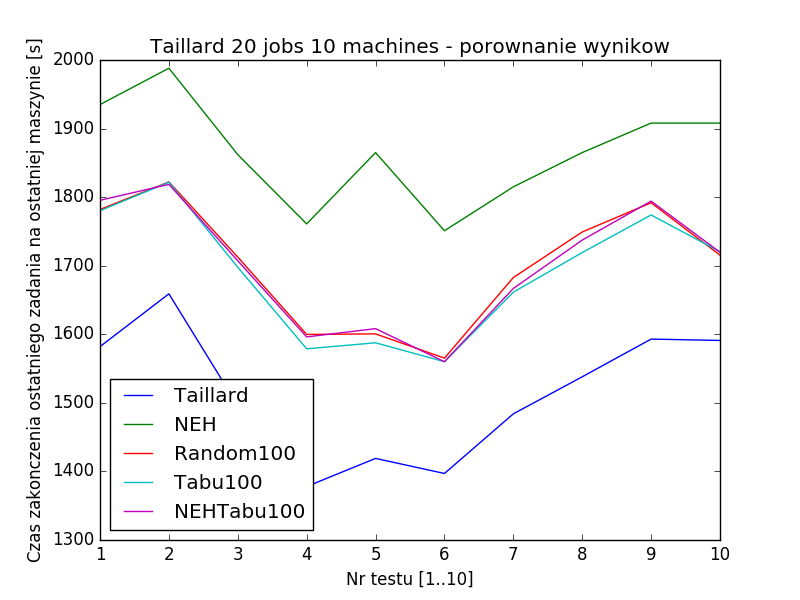
\includegraphics[scale=0.5]{test_taillard_20_wyniki.png}
\end{frame}

\begin{frame}
\frametitle{Eksperymenty obliczeniowe}	
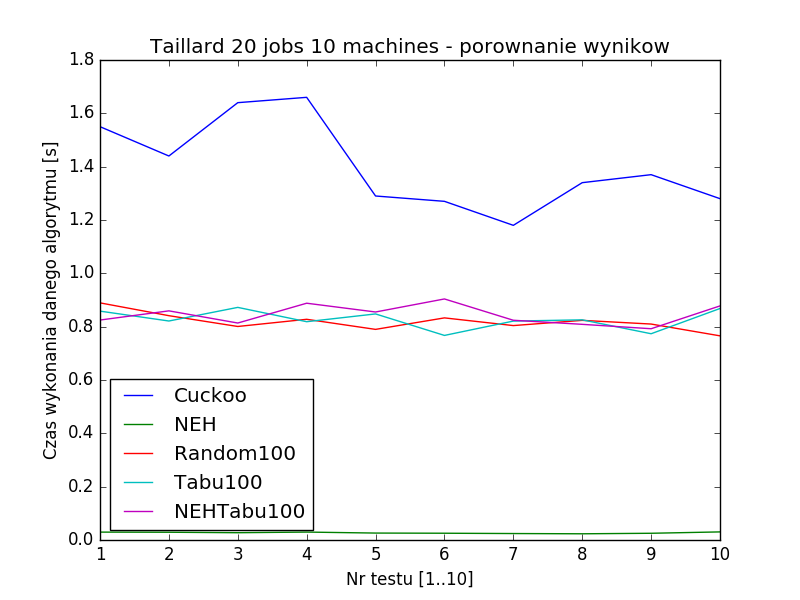
\includegraphics[scale=0.5]{test_taillard_20_czasy.png}
\end{frame}

%---------------------------------------------------------------------

\begin{frame}
\Huge{\centerline{Pytania?}}
\end{frame}


\begin{frame}
\Huge{\centerline{Odpowiedzi!}}
\end{frame}

%---------------------------------------------------------------------

\end{document} 